\chapter{Migratable Applications}
\label{chap:migratableapps}

In this chapter we introduce migration-friendly applications and pinpoint
common properties among them. These speculations almost inevitably lead
us towards coming up with a certain computation model for these
applications.
The functional and performance requirements of this computation model will
ask for certain features from a hypothetical migration framework. As the
takeaway from this chapter we will infer the goals that we must pursue
in designing Slope to address those requirements.

speculate api

possible usecases in distributed applications

design goals and important metrics

where do we need to be careful

say these are the things we need to do, lay out some requirements,
balance tradeoffs (e.g. access at source vs how quickly do the mig,
track allocs

\section{Migration-friendly applications}
Distributed applications refer to a large family of applications with
different functionalities and requirements. From distributed transactions
engines and RPC frameworks to data pipelines and graph processing systems,
we must identify the
applications which can naturally play along with the notion of migrating
slices of their work to their peers to achieve better load balancing.

However instead of taking a vertical slice of applications from this range
to target one of these domains, a horizontal slice possibly spanning
multiple of the domains can help us better identify the core
properties of migratable applications.

\subsection{Migratable partitions}

Figure \ref{fig:designgoalspluggable} shows our first sketch of a
migration-friendly application which consists of symmetric instances
running on the machines in a cluster. The application can internally
partition its units of work into partitions that can be operated or
managed either independently, or less strictly,
with well defined and infrequent cross-communication through APIs.
This partitioning scheme could be natural, like
partitioning user data data based on the user id, or it could be driven
by a pure need for load balancing, such as randomly sharding the data
in a transaction processing system.


\begin{figure}[t]
\centering

\ensurepdffromsvg{design-goals-pluggable.drawio}
\includegraphics[width=0.5\textwidth]{design-goals-pluggable.drawio}
\caption{
    The migration platform allows the already partitioned units of
    data/computation to be migrated across machines. Application partitions
    are the self-sufficient, independent units of work and therefore the
    migratable objects in this system.
}
\label{fig:designgoalspluggable}
\end{figure}

An immediate gain of the application from this model is load balancing,
while retaining locality of access and in case of repeated requests to
the applications, cache locality.
Given that the application can decompose its data and processing into
partitions that are small enough, it can use the migration platform to
spread
out its load evenly across the cluster. In time-sensitive applications
if the load is dynamic,
meaning the need to rebalance the workload arises frequently,
then the migration platform must also work in real-time.

In these applications each shard or partition will likely provide the
full API of the whole system. In Figure \ref{fig:designgoalspluggable},
if the workload did not contain partitions 2 and 3, then the only
    difference in the transition from top to bottom would have been the
    thin API wrapper around its partition which is responsible for tasks
    such as routing the requests to the correct machine. Otherwise
    Partition 1 would look like the whole application from the outside.

Therefore apart from the run-time load balancing benefit, the
    migration platform also simplifies a part of the development of the
    application: the system designer needs to program to an
    \emph{application partition}, as opposed to programming to the
    \emph{whole system}. This separation of concern,
    by definition breaks the dependency between how
    any shard handles a request to its API and what the rest of the
    platform does, including how request routing or replication is done
    in the application. Note that the need for request routing or
    replication are not implications of the partitioned computation
    model: we had to go distributed already to meet the requirements of
    the big workloads, but in a partitioned model we can think about those
    in isolation without propagating their complications to the
    core of the application.


\subsection{Migratability as a transport}
With certain performance qualifications, a migration framework can act as
an intra-cluster transport. Example use cases for such a transport arise
in application level (or layer 7 in OSI terms) routers in heterogeneous
computation environments. Figure \ref{fig:migrationtransport} depicts
a simple example of this use case. 

\begin{figure}[t]
\centering

\ensurepdffromsvg{migration-transport.drawio}
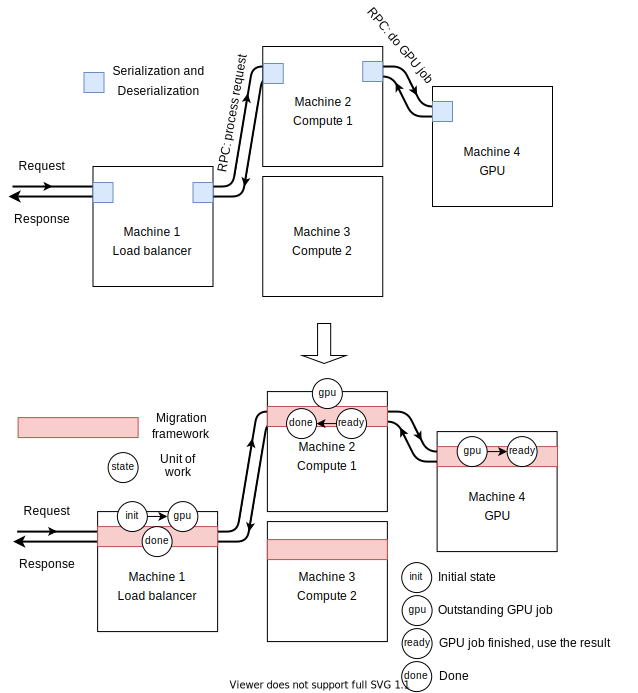
\includegraphics[width=0.5\textwidth]{migration-transport.drawio}
\caption{
    Using a migration platform as the transport in a system with
    application level routing/load balancing. The system needs to execute
    the data parallel computation portion of each task on the machine
    which has a GPU. A request/job is the
    migratable element in this scenario. Each request is independent
    from other requests. Each request is also self sufficient as its
    state identifies what action and by which machine type must be
    executed on the object. Each node executes its share of work
    on the request object based on its current state, updates the state,
    and sends it to the next hop based on the state.
}
\label{fig:migrationtransport}
\end{figure}


needs performance better than serialization

real-time

if have fast migraition, but have GPU or DB on certain nodes.



\section{Computation model and API}
\label{sec:api}
migratable objects are swarm-like types, not singletons

We want to be able to transform from A to B. Figure
\ref{fig:designgoalspluggable} shows how this idea will be look like on a high
level. Generally a requirement for routing the requests will be introduced.


\subsection{A section on how useful the programming model is}
E.g. what data structures can be used naturally in this model
Moved here from evaluation section
\subsection{Multi-threading support}

describe the \texttt{run()} function and describe the ``thread of execution''.
\TODO{...}

describe threading model

\TODO{figure for per core and how threads interact with them}

\TODO{fill}
Fundamentally every server has to be able to host an incoming object.
Since everything is async, this means that the object must know how to
"register" itself upon arrival in the remote node. Be it exposing a particular
api on a unix domain socket, or adding itself as an observer or worker to a blah.

each control plane has a fixed type

applications can intelligently use the time until ownership is transferred by
supporting read-only operations and even write operations with carefully
created static buffers that can contain unsupported (those that allocate/deallocate)
operations that the object has received after a call to initiate migration has
already been made.


\subsection{state machine}
task with gpu/accelerator friendly component

\subsection{listen and serve}
distributed key-value store


\section{Design goals}

Slope aims to provide a migration mechanism \CHECK{to allow applications to}
seamlessly move their data structures, and as a result, their corresponding
operations, across their instances.

The most important design goal of Slope is being pluggable in existing
applications which work with their data in a partitionable way. That means if
the system designer has already come up with a way to partition
application data and computation into units that can be run independently on 
possibly different machines, the task of integrating Slope into the system
to make its data
structures or more complex computation units migratable should be trivial.

To be more specific, we aim for zero modification to the internals of the
application and minimal addition to the API of the computation units just to
correctly define their behavior during their life cycle in Slope.

The migration delay which we define as the elapsed time since the start of the
migration of an object until it is successfully migrated is an important
performance metric in Slope. Clearly any application will prefer a smaller
end-to-end migration delay if every other metric is left unchanged. In contrast,
exceedingly large migration delays will interfere with the performance of
virtually all applications.

However, directly measuring this duration and pursuing its optimization
as the main performance goal may fail
\CHECK{} to reflect how the migration process impacts the application. Some
applications may prioritize responsiveness and would trade off some of their
throughput during the migration process to keep their tail latencies low.
Similarly an application may choose the opposite or any scenario in the middle.
Therefore it makes more sense to define migration performance from the view
point of the application based on how \emph{its} performance metrics degrade
as a result of the migration. Therefore while there is value in keeping the
migration delay small, we prioritize maximizing the \emph{usefulness} of the
application in the distributed setting during the migration.

\TODO{we explore these more in the evaluation section (how to define usefulness)}

